\section{Wolfram Mathematica}
\subsection{符号计算}
首先我们可以用 Mathematica 用于计算,众所周知 MMA 的符号计算是很强大的.
\begin{align}
    \wolfram{Series[Exp[x], {x, 0, 5}]}
\end{align}

\subsection{生成图片}
\subsubsection{二维图片}
MMA 图片测试,下面的这个绘图还是比较复杂的,于是我们使用MMA绘制,可以得
到\ref{MMA二维图形1}, \ref{MMA二维图形2}这两个绘图结果
\begin{bytes}
\wolframgraphics{
    ContourPlot[
    x^2/4 + y^2/3 == 5, {x, -5, 5}, {y, -5, 5},
    ContourStyle->{
        % 同样的,被latex注释的部分不会传入MMA
        % RGBColor["\#00C0A3"], 
        % 在传参的过程中,不要使用#,即使是\#,MMA也是会报错的。
        RGBColor[0.,0.7529411764705882,0.6392156862745098],
        Thickness[0.004]
    },
    AspectRatio->1, 
    AxesOrigin->{0,0}, 
    Axes->True,
    Frame->False,
    AxesStyle->Arrowheads[{0, 0.03}],
    AxesLabel->{"x", "y"}
]}{MMA2d1}
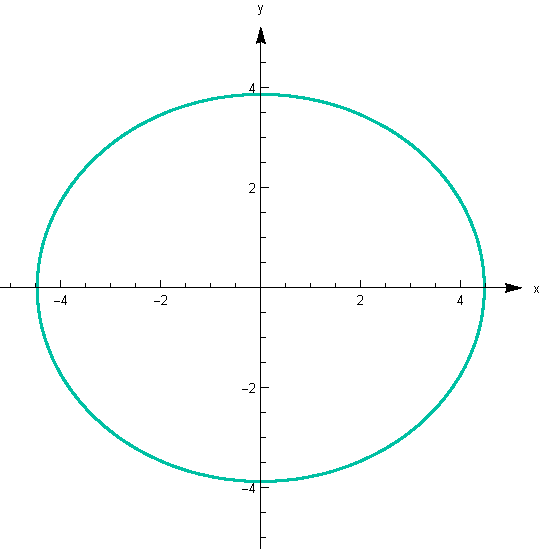
\includegraphics[scale=.7]{MMA2d1.pdf}
\end{bytes}

\begin{figure}[!htb]
    \centering
    \wolframgraphics{
		ContourPlot[
		x^2/4 + y^2/3 == 5, {x, -5, 5}, {y, -5, 5},
		ContourStyle->{
			% 同样的,被latex注释的部分不会传入MMA
			% RGBColor["\#00C0A3"], 
			% 在传参的过程中,不要使用#,即使是\#,MMA也是会报错的。
			RGBColor[0.,0.7529411764705882,0.6392156862745098],
			Thickness[0.004]
		},
		AspectRatio->1, 
		AxesOrigin->{0,0}, 
		Axes->True,
		Frame->False,
		AxesStyle->Arrowheads[{0, 0.03}],
		AxesLabel->{"x", "y"}
	]}{MMA2d1}
    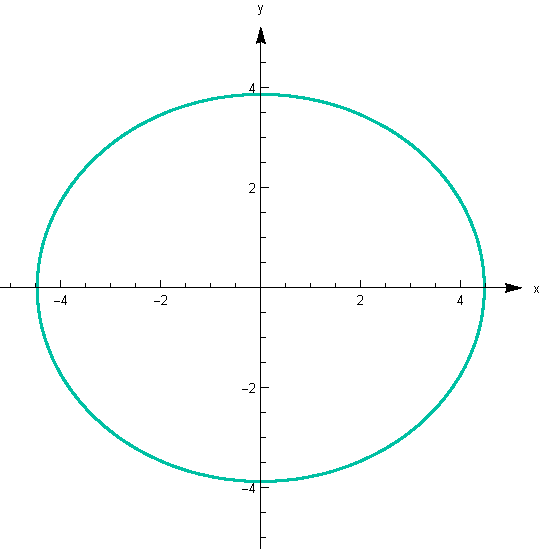
\includegraphics[scale=.7]{MMA2d1.pdf}
	\caption{MMA二维图形1}
	\label{MMA二维图形1}
\end{figure}

\begin{figure}[!htb]
    \centering
    \wolframgraphics{
    NumberLinePlot[
	    {Interval[{5, Infinity}], Interval[{2, 7}]}, 
	    AxesStyle->Arrowheads[{0, 0.03}]
    ]
    }{MMA2d2}
    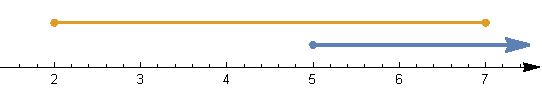
\includegraphics[scale=.7]{MMA2d2.pdf}
    \caption{MMA二维图形2}
    \label{MMA二维图形2}
\end{figure}

\subsubsection{三维图片}
二维的一些图形绘制了之后,自然要去绘制一些MMA中的3维对象了。下面就是
一些例子:
\begin{bytes}
\wolframgraphics{
    Arrow[Tube[
        BSplineCurve[{{0,0,0}, {.2,1,0.5},{2,1,1}}]
    ]]//Graphics3D}{MMA3d1}
\wolframgraphics{
    VectorPlot3D[
        {x, y, z}, {x, -1, 1}, 
        {y, -1, 1}, {z,-1, 1},
        PlotTheme->"Classic"
    ]}{MMA3d2}
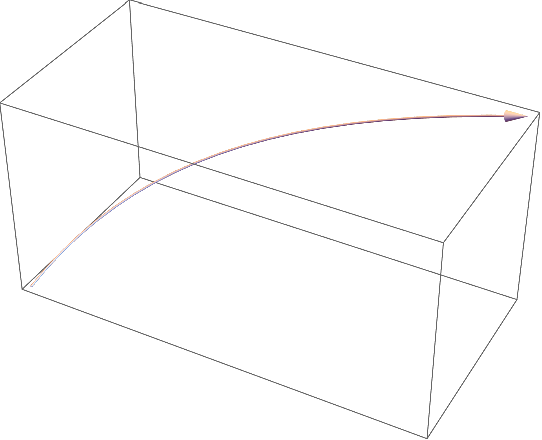
\includegraphics[scale=.7]{MMA3d1.pdf}
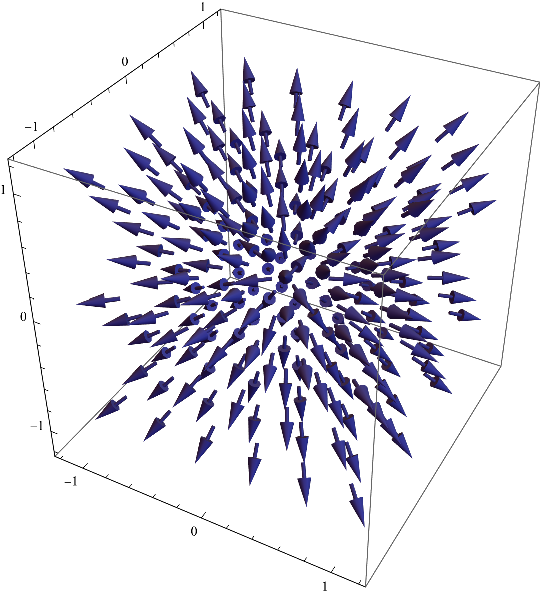
\includegraphics[scale=.7]{MMA3d2.pdf}
\end{bytes}

\begin{figure}[!htb]
    \centering
    \wolframgraphics{
        Arrow[Tube[
		    BSplineCurve[{{0,0,0}, {.2,1,0.5},{2,1,1}}]
        ]]//Graphics3D}{MMA3d1}
    \wolframgraphics{
        VectorPlot3D[
            {x, y, z}, {x, -1, 1}, 
            {y, -1, 1}, {z,-1, 1},
            PlotTheme->"Classic"
        ]}{MMA3d2}
    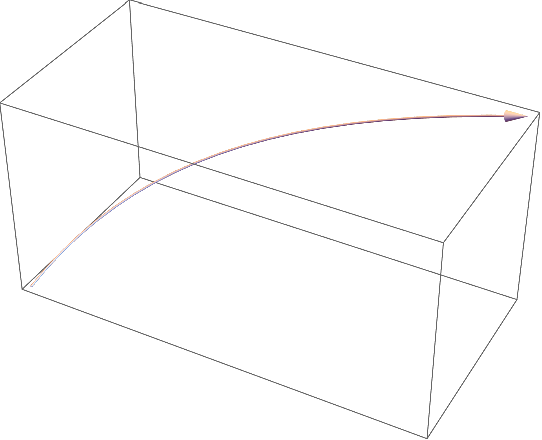
\includegraphics[scale=.7]{MMA3d1.pdf}
    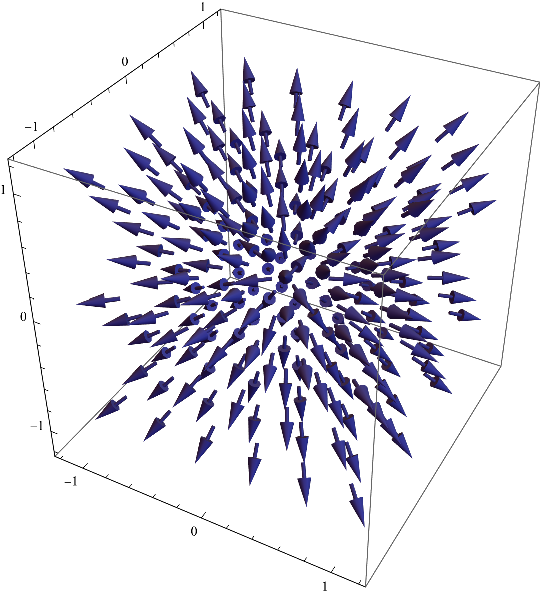
\includegraphics[scale=.7]{MMA3d2.pdf}
    \caption{MMA 三维图形}
    \label{MMA 三维图形}
\end{figure}

\subsection{微分方程}
这里肯定少不了我们的微分方程求解


\subsection{生成表格}
MMA还能够解方程,求根公式,输出表格等等.
